\chapter{Evaluation}
\label{eval}

\section{Introduction}
In this chapter the two implemented techniques will be evaluated under three read world workloads. In order to show the effect of each configuration parameter, multiple experiments have been designed and deployed. Table~\ref{des:tab:config} defines the configuration space. First, characteristics of workload will be discussed in Section~\ref{eval:workload}. Thereafter, there is separate section for each experiment. Finally, Section~\ref{eval:conc} concludes this chapter.

\section{Workload Characteristic}
\label{eval:workload}

DEBS 2014~\cite{debs2014} has been chosen as a real world workload to test the implementation. Each workload contains data from a random location of the original workload and replayed to feed Spark cluster. All experiments were run for one hour. Figure~\ref{eval:fig:workload} shows distribution of messages in three workloads which have been captured from Spark UI.
\begin{figure}
    \centering
      \begin{subfigure}[h]{\linewidth}
        \centering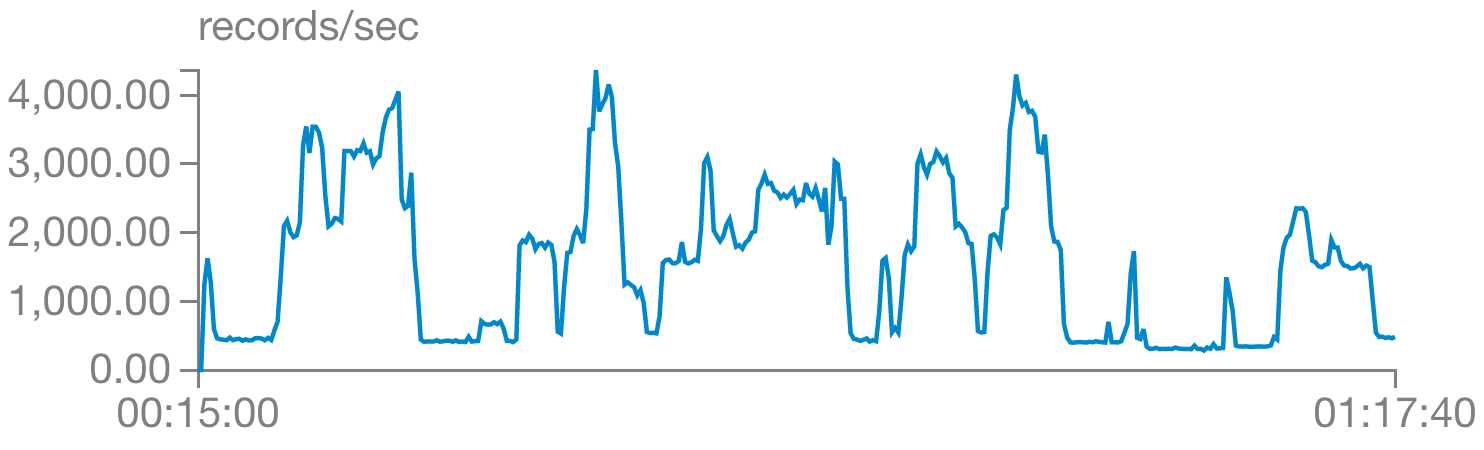
\includegraphics[scale=0.6]{workload1.png}
        \caption{Workload 1}
    \end{subfigure}
    \begin{subfigure}[h]{\linewidth}
        \centering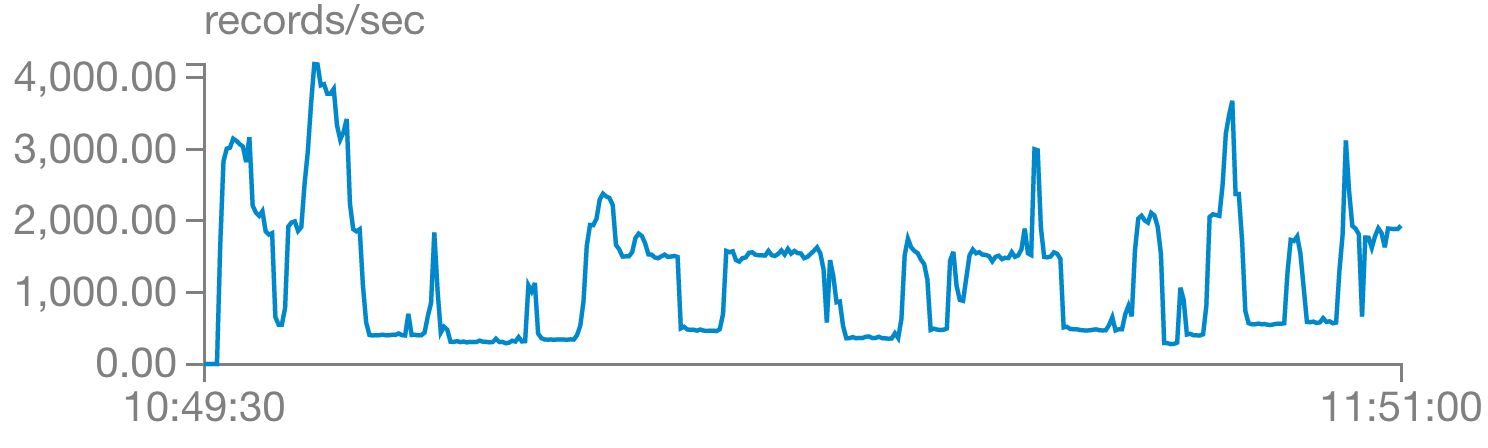
\includegraphics[scale=0.6]{workload2.png}
        \caption{Workload 2}
    \end{subfigure}
    \caption{Three Workloads of DEBS 2014}
    \label{eval:fig:workload}
\end{figure}

The workload involves sensors that measure energy consumption of devices. Each device is connected to one household which in turn is located in one house. This creates a hierarchy from house as parent of households and household as parent of devices. The workload asks to predict energy consumption per device, per household, and per house  for next window of time. The prediction runs over a sliding window of historical measurements which contains $n$ elements. Assuming $window$ variable contains $n$ elements of the history, Equation~\ref{eval:l:pred} defines how the predicted value is calculated.
\begin{equation}
\text{predicted value} = \frac{\text{average(window)} + \text{median(window)}}{2}
\label{eval:l:pred}
\end{equation}

In all experiments \emph{batch size} is set to 10 seconds. The cluster uses 24 executors with minimum of 4 executors that should be respected by Auto-Scaler. All experiments start with minimum number of executors -- 4 in this case -- and run for \emph{one} hour. In case any training is required to run the experiment, training data set is separated from the original workload dataset.

In order to make each workload CPU intensive enough, window size is changed for each workload. Table~\ref{eval:tab:history} defines the history window size for each workload.
\begin{table*}[h]
    \begin{tabular}{lc}
        \toprule
        \textbf{Workload} & \textbf{Window Size = $n$ }\\
        \midrule
        Workload 1 & 1650\\
        Workload 2 & 1900\\
        \bottomrule
    \end{tabular}
    \centering
    \caption{Workload Window Size}
    \label{eval:tab:history}
\end{table*}

\clearpage
\section{Experiment 1: Executor Strategy}
This experiment has been designed to illustrate the strategy of adding/removing executors when taking Scale-In or Scale-Out actions. Table~\ref{eval:tab:ex1} shows the configuration of this experiment.
\begin{table}[h]
    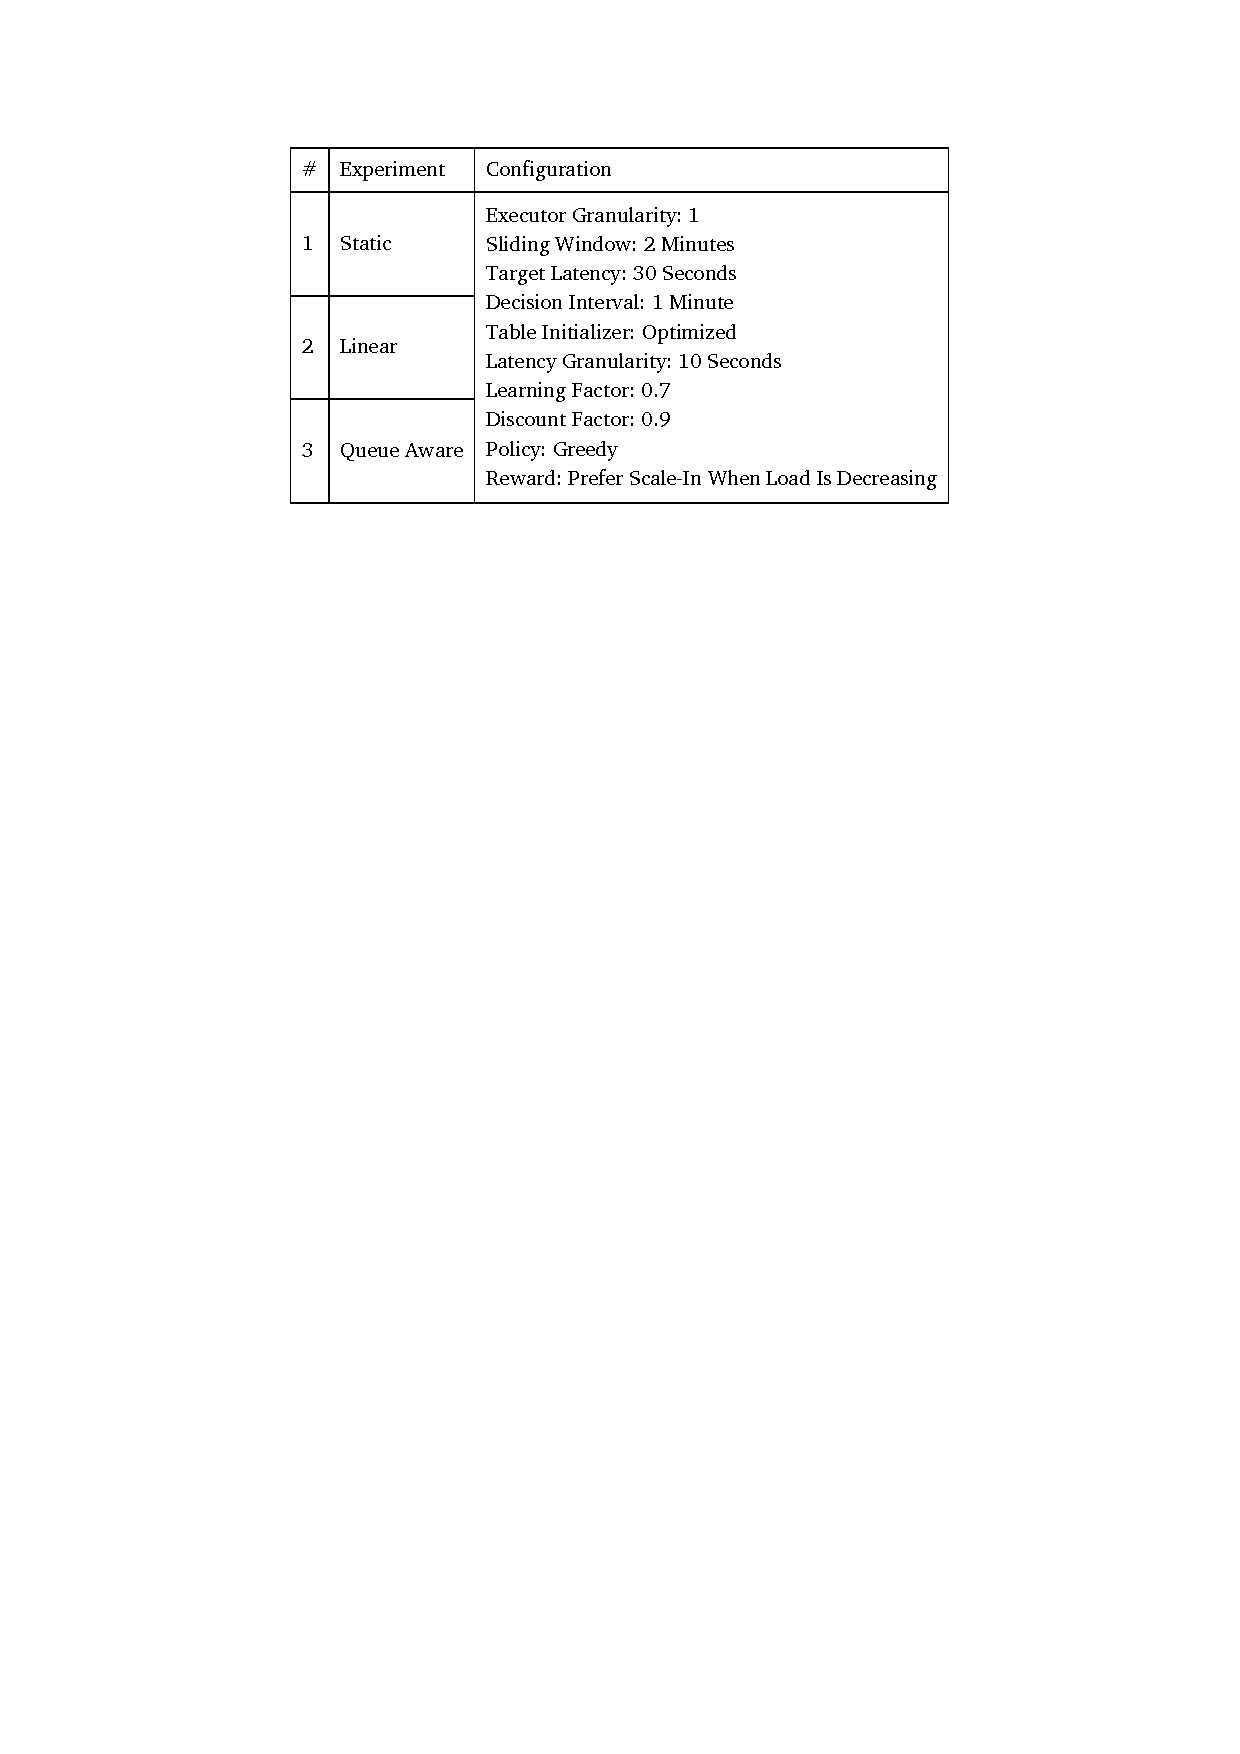
\includegraphics[clip,trim=3.6cm 21.18cm 2.75cm 2.5cm]{tables/ex1.pdf}
    \centering
    \caption{Executor Strategy Configuration Parameters}
    \label{eval:tab:ex1}
\end{table}

Figure~\ref{eval:f:e1:w1:lat},~\ref{eval:f:e1:w1:lat-c} depicts latency charts for first workload. Furthermore, Figure~\ref{eval:f:e1:w1:exec},~\ref{eval:f:e1:w1:exec-c} depicts the behavior of strategies regarding number of executors. Similarity, Figure~\ref{eval:f:e1:w2:lat},~\ref{eval:f:e1:w2:lat-c},~\ref{eval:f:e1:w2:exec} and~\ref{eval:f:e1:w2:exec-c} illustrates latency and executor charts for second workload.

\begin{figure}[!htbp]
\centering
\begin{gnuplot}[terminal=epslatex, terminaloptions=color colortext]
set terminal epslatex size 16cm,7.5cm
set key outside center top horizontal
set datafile separator ';'
set xdata time
set timefmt '%H:%M:%S'
set xr ['0:00:00':'1:00:00']
set yr [0:150]
set xtics '00:00:00',600 nomirror
set ytics 0,20 nomirror
set y2r [0:150]
set y2tics 0,20
set samples 50000 
unset mxtics
unset mytics
set grid ytics lc rgb "#bbbbbb" lw 1 lt 0
set grid xtics lc rgb "#bbbbbb" lw 1 lt 0
unset xl
set yl 'Latency (Seconds)'
plot 'ex/e1/w1/latency.csv' using 1:2 w l lc 'red' lw 4 smooth csplines t 'Static',\
'' using 1:3 w l lc 'blue' lw 4 smooth csplines t 'Linear',\
'' using 1:4 w l lc 'black' lw 4 smooth csplines t 'Q-Aware'
\end{gnuplot}
\caption{Executor Strategy -- Workload 1 -- Latency}
\label{eval:f:e1:w1:lat}
\end{figure}
\begin{figure}[!htbp]
	\centering
	\begin{minipage}[h]{\linewidth}
		\centering
		\begin{gnuplot}[terminal=epslatex, terminaloptions=color colortext]
			set terminal epslatex size 16cm,7.5cm
			set key outside center top horizontal
			set datafile separator ';'
            set key width -12
			set xr [0.5:3.5]
			set yr [0:150]
			set ytics 0,20 nomirror
			set y2r [0:150]
			set y2tics 0,20
			set boxwidth 0.3 absolute
			set style fill empty
			unset xl
            set grid ytics lc rgb "#bbbbbb" lw 1 lt 0
            set grid xtics lc rgb "#bbbbbb" lw 1 lt 0
			set yl 'Latency (Seconds)'
			plot 'ex/e1/w1/latency-c.csv' using 1:2:3:4:5:xticlabels(7) with candlesticks lc 'black' lw 4 t 'Min/Max/Percentiles',\
			'' using 1:6:6:6:6 with linespoints pt 5 lc 'black' lw 4 t 'Average',\
            30 dashtype 2 lc 'black' lw 4 t 'Target'
		\end{gnuplot}
		\caption{Executor Strategy -- Workload 1 -- Latency}
		\label{eval:f:e1:w1:lat-c}
	\end{minipage}\hfil
	\begin{minipage}[h]{\linewidth}
		\centering
		\begin{gnuplot}[terminal=epslatex, terminaloptions=color colortext]
			set terminal epslatex size 16cm,7.5cm
			set key outside center top horizontal
			set datafile separator ';'
			set xdata time
			set timefmt '%H:%M:%S'
			set xr ['0:00:00':'1:00:00']
			set yr [2:26]
			set y2r [2:26]
			set ytics 0,4 nomirror
			set xtics '00:00:00',600 nomirror
			set y2tics 0,4
			unset mxtics
			unset mytics
			unset xl
            set grid ytics lc rgb "#bbbbbb" lw 1 lt 0
            set grid xtics lc rgb "#bbbbbb" lw 1 lt 0
			set yl 'Number of Executors'
			plot 'ex/e1/w1/exec.csv' using 1:2 w l lc 'red' lw 4 t 'Static',\
			'' using 1:3 w l lc 'blue' lw 4 t 'Linear',\
			'' using 1:4 w l lc 'black' lw 4 t 'Q-Aware'
		\end{gnuplot}
		\caption{Executor Strategy -- Workload 1 -- Number of Executors}
		\label{eval:f:e1:w1:exec}
	\end{minipage}\hfil
	\begin{minipage}[h]{\linewidth}
		\centering
		\begin{gnuplot}[terminal=epslatex, terminaloptions=color colortext]
			set terminal epslatex size 16cm,7.5cm
			set key outside center top horizontal
			set datafile separator ';'
			set xr [0.5:3.5]
			set yr [2:26]
			set y2r [2:26]
			set ytics 0,4 nomirror
			set y2tics 0,4 nomirror
			set boxwidth 0.3 absolute
			set style fill empty
			unset xl
            set grid ytics lc rgb "#bbbbbb" lw 1 lt 0
            set grid xtics lc rgb "#bbbbbb" lw 1 lt 0
			set yl 'Number of Executors'
			plot 'ex/e1/w1/exec-c.csv' using 1:2:3:4:5:xticlabels(7) with candlesticks lc 'black' lw 4 t 'Min/Max/Percentiles',\
			'' using 1:6:6:6:6 with linespoints pt 5 lc 'black' lw 4 t 'Average' 
		\end{gnuplot}
		\caption{Executor Strategy -- Workload 1 -- Number of Executors}
		\label{eval:f:e1:w1:exec-c}
	\end{minipage}
\end{figure}
\begin{figure}[!htbp]
	\centering
	\begin{minipage}[h]{\linewidth}
		\centering
		\begin{gnuplot}[terminal=epslatex, terminaloptions=color colortext]
			set terminal epslatex size 16cm,7.5cm
			set key outside center top horizontal
			set datafile separator ';'
			set xdata time
			set timefmt '%H:%M:%S'
			set xr ['0:00:00':'1:00:00']
			set yr [0:170]
			set y2r [0:170]
			set xtics '00:00:00',600 nomirror
			set ytics 0,20 nomirror
			set y2tics 0,20
			unset mxtics
			unset mytics
			set samples 50000 
			unset xl
            set grid ytics lc rgb "#bbbbbb" lw 1 lt 0
            set grid xtics lc rgb "#bbbbbb" lw 1 lt 0
			set yl 'Latency (Seconds)'
			plot 'ex/e1/w2/latency.csv' using 1:2 w l lc 'red' lw 4 smooth csplines t 'Static',\
			'' using 1:3 w l lc 'blue' lw 4 smooth csplines t 'Linear',\
			'' using 1:4 w l lc 'black' lw 4 smooth csplines t 'Q-Aware'
		\end{gnuplot}
		\caption{Executor Strategy -- Workload 2 -- Latency}
		\label{eval:f:e1:w2:lat}
	\end{minipage}\hfil
	\begin{minipage}[h]{\linewidth}
		\centering
		\begin{gnuplot}[terminal=epslatex, terminaloptions=color colortext]
			set terminal epslatex size 16cm,7.5cm
			set key outside center top horizontal
			set datafile separator ';'
            set key width -12
			set xr [0.5:3.5]
			set yr [0:170]
			set y2r [0:170]
			set ytics nomirror
			set y2tics 0,20
			set boxwidth 0.3 absolute
			set style fill empty
			unset xl
            set grid ytics lc rgb "#bbbbbb" lw 1 lt 0
            set grid xtics lc rgb "#bbbbbb" lw 1 lt 0
			set yl 'Latency (Seconds)'
			plot 'ex/e1/w2/latency-c.csv' using 1:2:3:4:5:xticlabels(7) with candlesticks lc 'black' lw 4 t 'Min/Max/Percentiles',\
			'' using 1:6:6:6:6 with linespoints pt 5 lc 'black' lw 4 t 'Average',\
            30 dashtype 2 lc 'black' lw 4 t 'Target'
		\end{gnuplot}
		\caption{Executor Strategy -- Workload 2 -- Latency}
		\label{eval:f:e1:w2:lat-c}
	\end{minipage}\hfil
	\begin{minipage}[h]{\linewidth}
		\centering
		\begin{gnuplot}[terminal=epslatex, terminaloptions=color colortext]
			set terminal epslatex size 16cm,7.5cm
			set key outside center top horizontal
			set datafile separator ';'
			set xdata time
			set timefmt '%H:%M:%S'
			set xr ['0:00:00':'1:00:00']
			set yr [2:26]
			set y2r [2:26]
			set xtics '00:00:00',600 nomirror
			set ytics 0,4 nomirror
			set y2tics 0,4
			unset mxtics
			unset mytics
			unset xl
            set grid ytics lc rgb "#bbbbbb" lw 1 lt 0
            set grid xtics lc rgb "#bbbbbb" lw 1 lt 0
			set yl 'Number of Executors'
			plot 'ex/e1/w2/exec.csv' using 1:2 w l lc 'red' lw 4 t 'Static',\
			'' using 1:3 w l lc 'blue' lw 4 t 'Linear',\
			'' using 1:4 w l lc 'black' lw 4 t 'Q-Aware'
		\end{gnuplot}
		\caption{Executor Strategy -- Workload 2 -- Number of Executors}
		\label{eval:f:e1:w2:exec}
	\end{minipage}
\end{figure}
\begin{figure}[!htbp]
\centering
\begin{gnuplot}[terminal=epslatex, terminaloptions=color colortext]
set terminal epslatex size 16cm,7.5cm
set key outside center top horizontal
set datafile separator ';'
set xr [0.5:3.5]
set yr [2:26]
set ytics 0,4 nomirror
set y2r [2:26]
set y2tics 0,4
set boxwidth 0.3 absolute
set style fill empty
unset xl
set grid ytics lc rgb "#bbbbbb" lw 1 lt 0
set grid xtics lc rgb "#bbbbbb" lw 1 lt 0
set yl 'Number of Executors'
plot 'ex/e1/w2/exec-c.csv' using 1:2:3:4:5:xticlabels(7) with candlesticks lc 'black' lw 4 t 'Min/Max/Percentiles','' using 1:6:6:6:6 with linespoints pt 5 lc 'black' lw 4 t 'Average' 
\end{gnuplot}
\caption{Executor Strategy -- Workload 2 -- Number of Executors}
\label{eval:f:e1:w2:exec-c}
\end{figure}
\FloatBarrier
\subsection{Conclusion}
As depicted in last section, for Workload 1, Static strategy performs slightly better than Queue Aware strategy. Both of them were able reach target latency to some degree, though they are still above target latency. However, for Workload 2 Queue Aware strategy outperforms all other strategies, since Static and Linear strategies violate target latency.

It can be speculated that Queue Aware strategy is the best strategy amongst three strategies. However, it can't be proven now. More experiments shall be done. Thus, for next set of experiments Queue Aware strategy is chosen to be evaluated extensively. Furthermore, the conclusion is only based on two workloads and it can't be generalized.
\clearpage
\section{Experiment 2: History Window}
This experiment has been designed to illustrate the effect of history window on quality of decision made by Auto-Scaler. Table~\ref{eval:tab:ex2} shows the configuration of this experiment.
\begin{table}[h]
    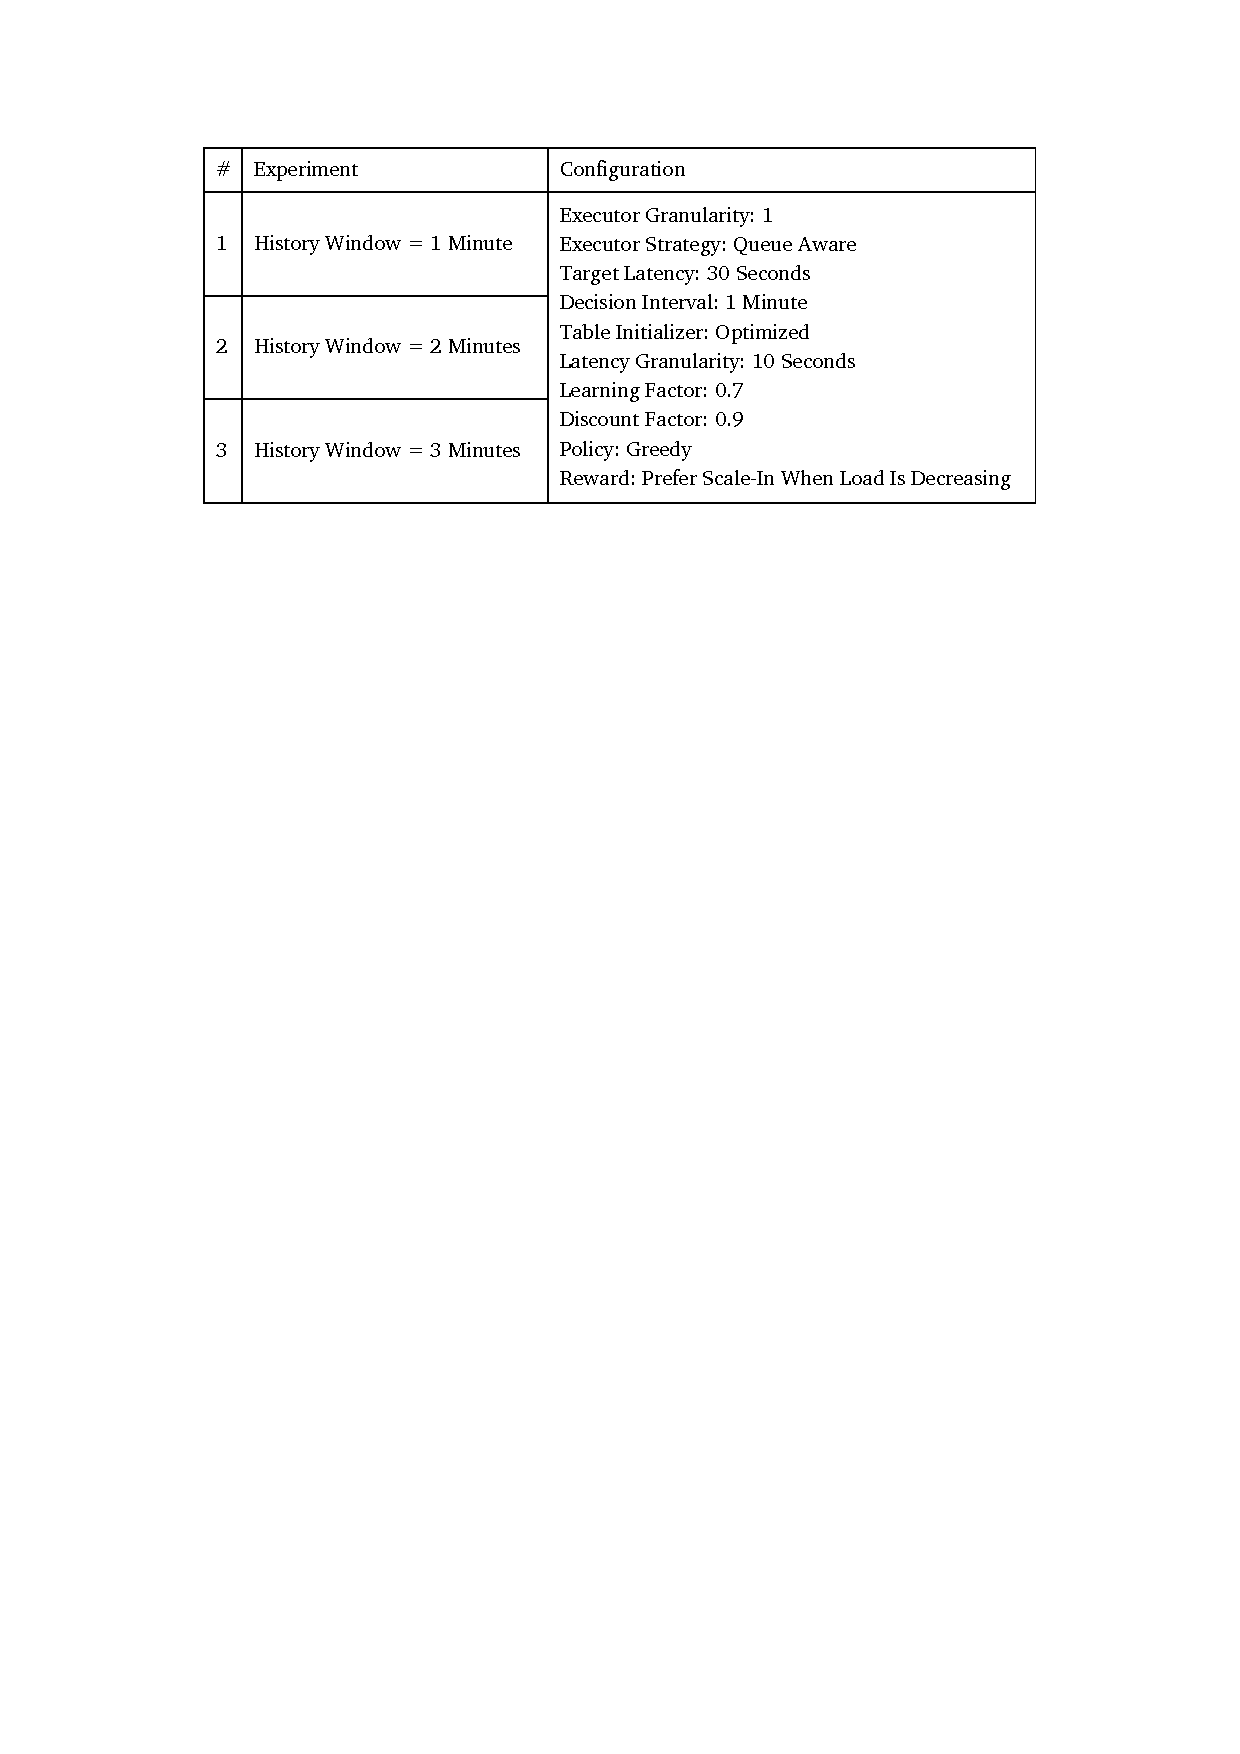
\includegraphics[clip,trim=3.3cm 21.18cm 3.25cm 2.5cm]{tables/ex2.pdf}
    \centering
    \caption{History Window Configuration Parameters}
    \label{eval:tab:ex2}
\end{table}

Figures~\ref{eval:f:e2:w1:lat},~\ref{eval:f:e2:w1:lat-c},~\ref{eval:f:e2:w1:exec} and ~\ref{eval:f:e2:w1:exec-c} illustrates latency and executor charts for Workload 1. Figures~\ref{eval:f:e2:w2:lat},~\ref{eval:f:e2:w2:lat-c},~\ref{eval:f:e2:w2:exec} and~\ref{eval:f:e2:w2:exec-c} illustrates latency and executor charts for Workload 2.

\begin{figure}[!htbp]
    \centering
    \begin{gnuplot}[terminal=epslatex, terminaloptions=color colortext]
        set terminal epslatex size 16cm,7.5cm
        set key outside center top horizontal
        set datafile separator ';'
        set xdata time
        set timefmt '%H:%M:%S'
        set xr ['0:00:00':'1:00:00']
        set yr [0:110]
        set xtics '00:00:00',600 nomirror
        set ytics 0,20 nomirror
        set y2r [0:110]
        set y2tics 0,20
        set samples 50000 
        unset mxtics
        unset mytics
        unset xl
        set grid ytics lc rgb "#bbbbbb" lw 1 lt 0
        set grid xtics lc rgb "#bbbbbb" lw 1 lt 0
        set yl 'Latency (Seconds)'
        plot 'ex/e2/w1/latency.csv' using 1:2 w l lc 'red' lw 4 smooth csplines t '1 Min',\
        '' using 1:3 w l lc 'blue' lw 4 smooth csplines t '2 Min',\
        '' using 1:4 w l lc 'black' lw 4 smooth csplines t '3 Min'
    \end{gnuplot}
    \caption{History Window -- Workload 1 -- Latency}
    \label{eval:f:e2:w1:lat}
\end{figure}
\begin{figure}[!htbp]
    \centering
    \begin{minipage}[h]{\linewidth}
        \centering
        \begin{gnuplot}[terminal=epslatex, terminaloptions=color colortext]
            set terminal epslatex size 16cm,7.5cm
            set key outside center top horizontal
            set datafile separator ';'
            set key width -12
            set xr [0.5:3.5]
            set yr [0:110]
            set ytics 0,20 nomirror
            set y2r [0:110]
            set y2tics 0,20
            set boxwidth 0.3 absolute
            set style fill empty
            unset xl
            set grid ytics lc rgb "#bbbbbb" lw 1 lt 0
            set grid xtics lc rgb "#bbbbbb" lw 1 lt 0
            set yl 'Latency (Seconds)'
            plot 'ex/e2/w1/latency-c.csv' using 1:2:3:4:5:xticlabels(7) with candlesticks lc 'black' lw 4 t 'Min/Max/Percentiles',\
            '' using 1:6:6:6:6 with linespoints pt 5 lc 'black' lw 4 t 'Average',\
            30 dashtype 2 lc 'black' lw 4 t 'Target'
        \end{gnuplot}
        \caption{History Window -- Workload 1 -- Latency}
        \label{eval:f:e2:w1:lat-c}
    \end{minipage}\hfil
    \begin{minipage}[h]{\linewidth}
        \centering
        \begin{gnuplot}[terminal=epslatex, terminaloptions=color colortext]
            set terminal epslatex size 16cm,7.5cm
            set key outside center top horizontal
            set datafile separator ';'
            set xdata time
            set timefmt '%H:%M:%S'
            set xr ['0:00:00':'1:00:00']
            set yr [2:26]
            set y2r [2:26]
            set ytics 0,4 nomirror
            set xtics '00:00:00',600 nomirror
            set y2tics 0,4
            unset mxtics
            unset mytics
            unset xl
            set grid ytics lc rgb "#bbbbbb" lw 1 lt 0
            set grid xtics lc rgb "#bbbbbb" lw 1 lt 0
            set yl 'Number of Executors'
            plot 'ex/e2/w1/exec.csv' using 1:2 w l lc 'red' lw 4 t '1 Min',\
            '' using 1:3 w l lc 'blue' lw 4 t '2 Min',\
            '' using 1:4 w l lc 'black' lw 4 t '3 Min'
        \end{gnuplot}
        \caption{History Window -- Workload 1 -- Number of Executors}
        \label{eval:f:e2:w1:exec}
    \end{minipage}\hfil
    \begin{minipage}[h]{\linewidth}
        \centering
        \begin{gnuplot}[terminal=epslatex, terminaloptions=color colortext]
            set terminal epslatex size 16cm,7.5cm
            set key outside center top horizontal
            set datafile separator ';'
            set xr [0.5:3.5]
            set yr [2:26]
            set y2r [2:26]
            set ytics 0,4 nomirror
            set y2tics 0,4 nomirror
            set boxwidth 0.3 absolute
            set style fill empty
            unset xl
            set grid ytics lc rgb "#bbbbbb" lw 1 lt 0
            set grid xtics lc rgb "#bbbbbb" lw 1 lt 0
            set yl 'Number of Executors'
            plot 'ex/e2/w1/exec-c.csv' using 1:2:3:4:5:xticlabels(7) with candlesticks lc 'black' lw 4 t 'Min/Max/Percentiles',\
            '' using 1:6:6:6:6 with linespoints pt 5 lc 'black' lw 4 t 'Average' 
        \end{gnuplot}
        \caption{History Window -- Workload 1 -- Number of Executors}
        \label{eval:f:e2:w1:exec-c}
    \end{minipage}
\end{figure}
\begin{figure}[!htbp]
    \centering
    \begin{minipage}[h]{\linewidth}
        \centering
        \begin{gnuplot}[terminal=epslatex, terminaloptions=color colortext]
            set terminal epslatex size 16cm,7.5cm
            set key outside center top horizontal
            set datafile separator ';'
            set xdata time
            set timefmt '%H:%M:%S'
            set xr ['0:00:00':'1:00:00']
            set yr [0:130]
            set y2r [0:130]
            set xtics '00:00:00',600 nomirror
            set ytics 0,20 nomirror
            set y2tics 0,20
            unset mxtics
            unset mytics
            set samples 50000 
            unset xl
            set grid ytics lc rgb "#bbbbbb" lw 1 lt 0
            set grid xtics lc rgb "#bbbbbb" lw 1 lt 0
            set yl 'Latency (Seconds)'
            plot 'ex/e2/w2/latency.csv' using 1:2 w l lc 'red' lw 4 smooth csplines t '1 Min',\
            '' using 1:3 w l lc 'blue' lw 4 smooth csplines t '2 Min',\
            '' using 1:4 w l lc 'black' lw 4 smooth csplines t '3 Min'
        \end{gnuplot}
        \caption{History Window -- Workload 2 -- Latency}
        \label{eval:f:e2:w2:lat}
    \end{minipage}\hfil
    \begin{minipage}[h]{\linewidth}
        \centering
        \begin{gnuplot}[terminal=epslatex, terminaloptions=color colortext]
            set terminal epslatex size 16cm,7.5cm
            set key outside center top horizontal
            set datafile separator ';'
            set key width -12
            set xr [0.5:3.5]
            set yr [0:130]
            set y2r [0:130]
            set ytics nomirror
            set y2tics 0,20
            set boxwidth 0.3 absolute
            set style fill empty
            unset xl
            set grid ytics lc rgb "#bbbbbb" lw 1 lt 0
            set grid xtics lc rgb "#bbbbbb" lw 1 lt 0
            set yl 'Latency (Seconds)'
            plot 'ex/e2/w2/latency-c.csv' using 1:2:3:4:5:xticlabels(7) with candlesticks lc 'black' lw 4 t 'Min/Max/Percentiles',\
            '' using 1:6:6:6:6 with linespoints pt 5 lc 'black' lw 4 t 'Average',\
            30 dashtype 2 lc 'black' lw 4 t 'Target'
        \end{gnuplot}
        \caption{History Window -- Workload 2 -- Latency}
        \label{eval:f:e2:w2:lat-c}
    \end{minipage}\hfil
    \begin{minipage}[h]{\linewidth}
        \centering
        \begin{gnuplot}[terminal=epslatex, terminaloptions=color colortext]
            set terminal epslatex size 16cm,7.5cm
            set key outside center top horizontal
            set datafile separator ';'
            set xdata time
            set timefmt '%H:%M:%S'
            set xr ['0:00:00':'1:00:00']
            set yr [2:26]
            set y2r [2:26]
            set xtics '00:00:00',600 nomirror
            set ytics 0,4 nomirror
            set y2tics 0,4
            unset mxtics
            unset mytics
            unset xl
            set grid ytics lc rgb "#bbbbbb" lw 1 lt 0
            set grid xtics lc rgb "#bbbbbb" lw 1 lt 0
            set yl 'Number of Executors'
            plot 'ex/e2/w2/exec.csv' using 1:2 w l lc 'red' lw 4 t '1 Min',\
            '' using 1:3 w l lc 'blue' lw 4 t '2 Min',\
            '' using 1:4 w l lc 'black' lw 4 t '3 Min'
        \end{gnuplot}
        \caption{History Window -- Workload 2 -- Number of Executors}
        \label{eval:f:e2:w2:exec}
    \end{minipage}
\end{figure}
\begin{figure}[!htbp]
    \centering
    \begin{gnuplot}[terminal=epslatex, terminaloptions=color colortext]
        set terminal epslatex size 16cm,7.5cm
        set key outside center top horizontal
        set datafile separator ';'
        set xr [0.5:3.5]
        set yr [2:26]
        set ytics 0,4 nomirror
        set y2r [2:26]
        set y2tics 0,4
        set boxwidth 0.3 absolute
        set style fill empty
        unset xl
        set grid ytics lc rgb "#bbbbbb" lw 1 lt 0
        set grid xtics lc rgb "#bbbbbb" lw 1 lt 0
        set yl 'Number of Executors'
        plot 'ex/e2/w2/exec-c.csv' using 1:2:3:4:5:xticlabels(7) with candlesticks lc 'black' lw 4 t 'Min/Max/Percentiles','' using 1:6:6:6:6 with linespoints pt 5 lc 'black' lw 4 t 'Average' 
    \end{gnuplot}
    \caption{History Window -- Workload 2 -- Number of Executors}
    \label{eval:f:e2:w2:exec-c}
\end{figure}
\FloatBarrier
\subsection{Conclusion}
For Workload 1, three-minute history window leads to better latency albeit with slightly more executors. However, for second workload two-minute window outperforms both one and three minute windows.

Also note that, short history window (like one-minute) makes Auto-Scaler too sensitive to noisy workloads. This can be confirmed by Figure~\ref{eval:f:e2:w2:exec}. As depicted, one-minute history window suffers from zig-zag decisions when it reaches 24 executors. Two-minute window to some degree suffers from this issue as well. However, three-minute window is resistant to this issue.

In general, history window of two minutes shows better results than the others. Thus, for rest of the experiments this window size will be used.
\clearpage
\section{Experiment 3: Decision Interval}
The Auto-Scaler implemented in thesis makes decisions in intervals defined by \lstinline|decisionInterval| parameter. This experiment has been designed to illustrate the effect of this parameter on behvaior of the Auto-Scaler. Table~\ref{eval:tab:ex3} shows the configuration of this experiment.
\begin{table}[h]
    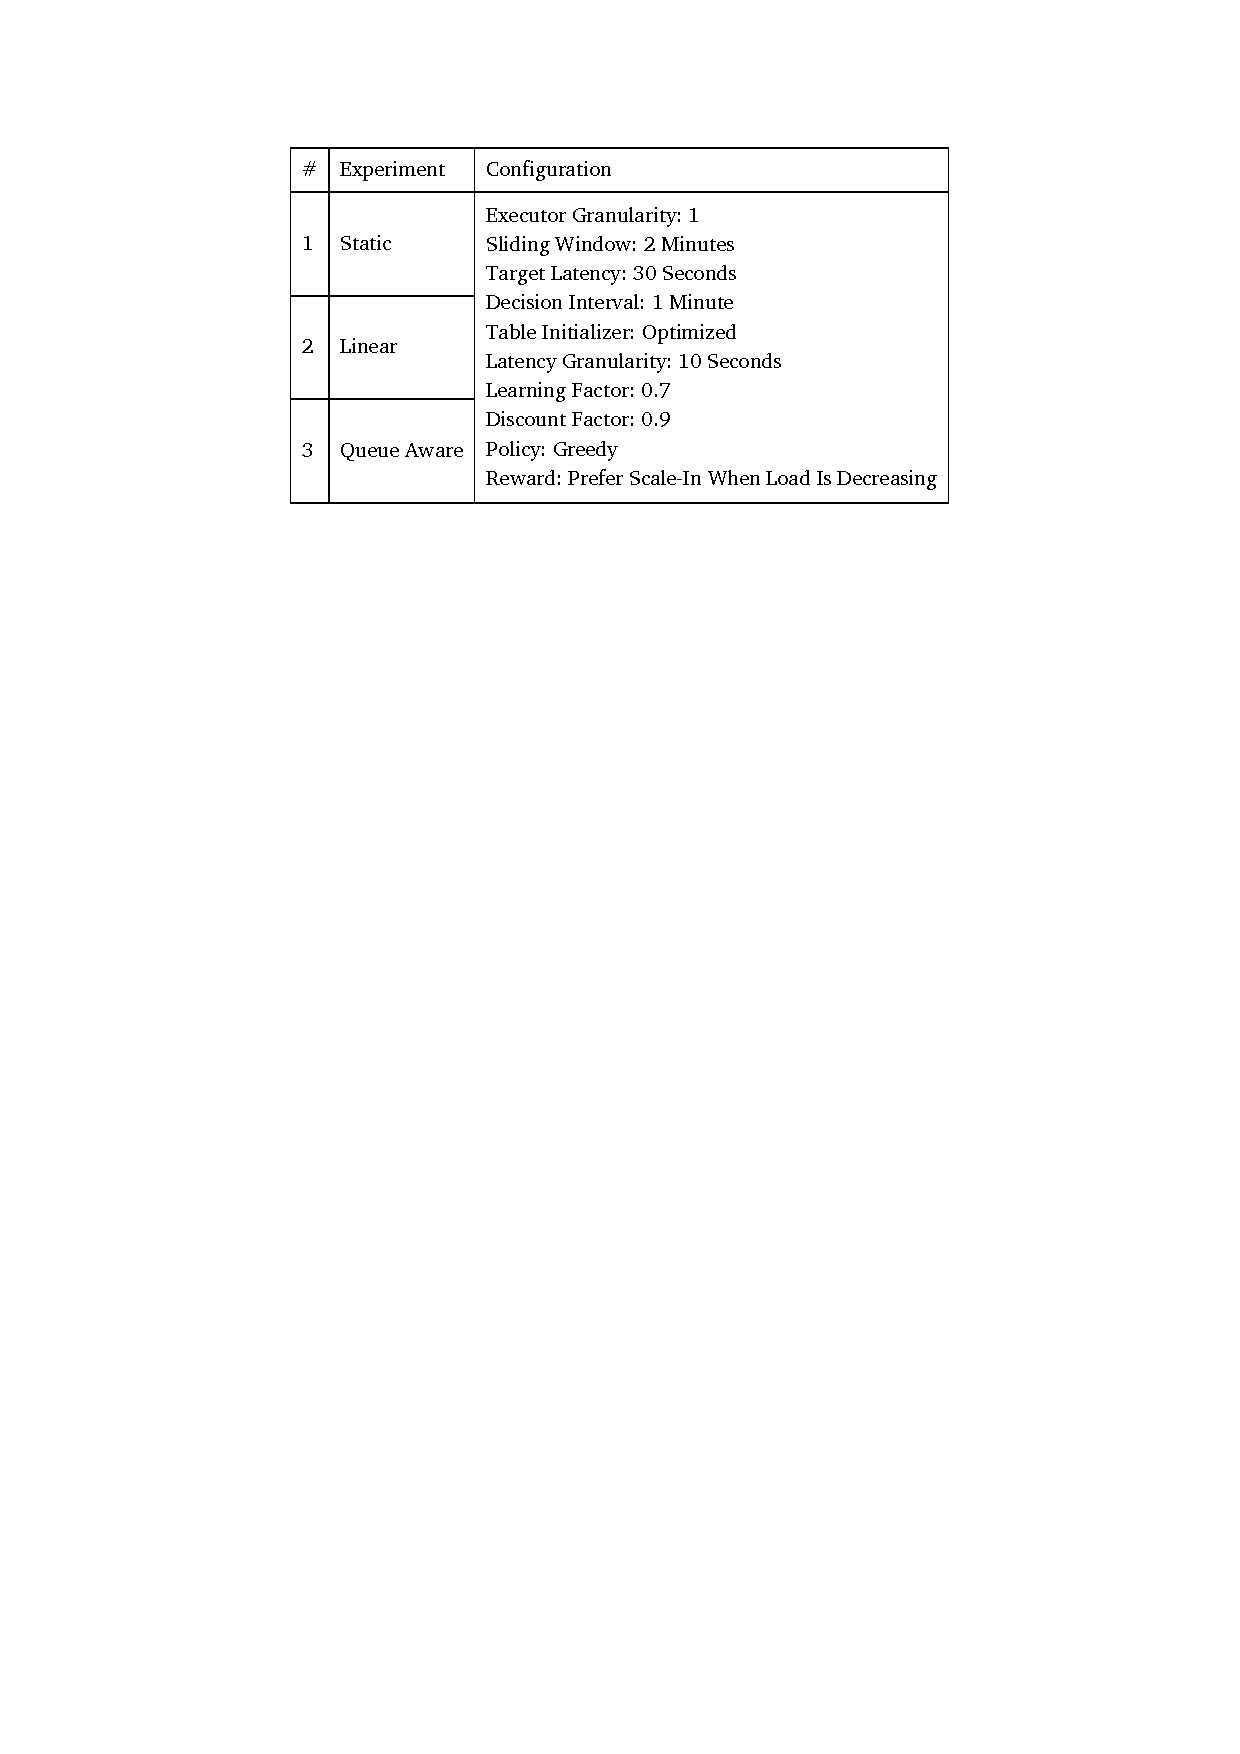
\includegraphics[clip,trim=3.3cm 21.18cm 3.25cm 2.5cm]{tables/ex3.pdf}
    \centering
    \caption{Decision Interval Configuration Parameters}
    \label{eval:tab:ex3}
\end{table}

Figures~\ref{eval:f:e3:w1:lat},~\ref{eval:f:e3:w1:lat-c},~\ref{eval:f:e3:w1:exec} and ~\ref{eval:f:e3:w1:exec-c} illustrates latency and executor charts for Workload 1. Figures~\ref{eval:f:e3:w2:lat},~\ref{eval:f:e3:w2:lat-c},~\ref{eval:f:e3:w2:exec} and~\ref{eval:f:e3:w2:exec-c} illustrates latency and executor charts for Workload 2.

\begin{figure}[!htbp]
    \centering
    \begin{gnuplot}[terminal=epslatex, terminaloptions=color colortext]
        set terminal epslatex size 16cm,7.5cm
        set key outside center top horizontal
        set datafile separator ';'
        set xdata time
        set timefmt '%H:%M:%S'
        set xr ['0:00:00':'1:00:00']
        set yr [0:110]
        set xtics '00:00:00',600 nomirror
        set ytics 0,20 nomirror
        set y2r [0:110]
        set y2tics 0,20
        set samples 50000 
        unset mxtics
        unset mytics
        unset xl
        set grid ytics lc rgb "#bbbbbb" lw 1 lt 0
        set grid xtics lc rgb "#bbbbbb" lw 1 lt 0
        set yl 'Latency (Seconds)'
        plot 'ex/e3/w1/latency.csv' using 1:2 w l lc 'red' lw 4 smooth csplines t '1 Min',\
        '' using 1:3 w l lc 'blue' lw 4 smooth csplines t '2 Min',\
        '' using 1:4 w l lc 'black' lw 4 smooth csplines t '3 Min'
    \end{gnuplot}
    \caption{Decision Interval -- Workload 1 -- Latency}
    \label{eval:f:e3:w1:lat}
\end{figure}
\begin{figure}[!htbp]
    \centering
    \begin{minipage}[h]{\linewidth}
        \centering
        \begin{gnuplot}[terminal=epslatex, terminaloptions=color colortext]
            set terminal epslatex size 16cm,7.5cm
            set key outside center top horizontal
            set datafile separator ';'
            set key width -12
            set xr [0.5:3.5]
            set yr [0:110]
            set ytics 0,20 nomirror
            set y2r [0:110]
            set y2tics 0,20
            set boxwidth 0.3 absolute
            set style fill empty
            unset xl
            set grid ytics lc rgb "#bbbbbb" lw 1 lt 0
            set grid xtics lc rgb "#bbbbbb" lw 1 lt 0
            set yl 'Latency (Seconds)'
            plot 'ex/e3/w1/latency-c.csv' using 1:2:3:4:5:xticlabels(7) with candlesticks lc 'black' lw 4 t 'Min/Max/Percentiles',\
            '' using 1:6:6:6:6 with linespoints pt 5 lc 'black' lw 4 t 'Average',\
            30 dashtype 2 lc 'black' lw 4 t 'Target'
        \end{gnuplot}
        \caption{Decision Interval -- Workload 1 -- Latency}
        \label{eval:f:e3:w1:lat-c}
    \end{minipage}\hfil
    \begin{minipage}[h]{\linewidth}
        \centering
        \begin{gnuplot}[terminal=epslatex, terminaloptions=color colortext]
            set terminal epslatex size 16cm,7.5cm
            set key outside center top horizontal
            set datafile separator ';'
            set xdata time
            set timefmt '%H:%M:%S'
            set xr ['0:00:00':'1:00:00']
            set yr [2:26]
            set y2r [2:26]
            set ytics 0,4 nomirror
            set xtics '00:00:00',600 nomirror
            set y2tics 0,4
            unset mxtics
            unset mytics
            unset xl
            set grid ytics lc rgb "#bbbbbb" lw 1 lt 0
            set grid xtics lc rgb "#bbbbbb" lw 1 lt 0
            set yl 'Number of Executors'
            plot 'ex/e3/w1/exec.csv' using 1:2 w l lc 'red' lw 4 t '1 Min',\
            '' using 1:3 w l lc 'blue' lw 4 t '2 Min',\
            '' using 1:4 w l lc 'black' lw 4 t '3 Min'
        \end{gnuplot}
        \caption{Decision Interval -- Workload 1 -- Number of Executors}
        \label{eval:f:e3:w1:exec}
    \end{minipage}\hfil
    \begin{minipage}[h]{\linewidth}
        \centering
        \begin{gnuplot}[terminal=epslatex, terminaloptions=color colortext]
            set terminal epslatex size 16cm,7.5cm
            set key outside center top horizontal
            set datafile separator ';'
            set xr [0.5:3.5]
            set yr [2:26]
            set y2r [2:26]
            set ytics 0,4 nomirror
            set y2tics 0,4 nomirror
            set boxwidth 0.3 absolute
            set style fill empty
            unset xl
            set grid ytics lc rgb "#bbbbbb" lw 1 lt 0
            set grid xtics lc rgb "#bbbbbb" lw 1 lt 0
            set yl 'Number of Executors'
            plot 'ex/e3/w1/exec-c.csv' using 1:2:3:4:5:xticlabels(7) with candlesticks lc 'black' lw 4 t 'Min/Max/Percentiles',\
            '' using 1:6:6:6:6 with linespoints pt 5 lc 'black' lw 4 t 'Average' 
        \end{gnuplot}
        \caption{Decision Interval -- Workload 1 -- Number of Executors}
        \label{eval:f:e3:w1:exec-c}
    \end{minipage}
\end{figure}
\begin{figure}[!htbp]
    \centering
    \begin{minipage}[h]{\linewidth}
        \centering
        \begin{gnuplot}[terminal=epslatex, terminaloptions=color colortext]
            set terminal epslatex size 16cm,7.5cm
            set key outside center top horizontal
            set datafile separator ';'
            set xdata time
            set timefmt '%H:%M:%S'
            set xr ['0:00:00':'1:00:00']
            set yr [0:130]
            set y2r [0:130]
            set xtics '00:00:00',600 nomirror
            set ytics 0,20 nomirror
            set y2tics 0,20
            unset mxtics
            unset mytics
            set samples 50000 
            unset xl
            set grid ytics lc rgb "#bbbbbb" lw 1 lt 0
            set grid xtics lc rgb "#bbbbbb" lw 1 lt 0
            set yl 'Latency (Seconds)'
            plot 'ex/e3/w2/latency.csv' using 1:2 w l lc 'red' lw 4 smooth csplines t '1 Min',\
            '' using 1:3 w l lc 'blue' lw 4 smooth csplines t '2 Min',\
            '' using 1:4 w l lc 'black' lw 4 smooth csplines t '3 Min'
        \end{gnuplot}
        \caption{Decision Interval -- Workload 2 -- Latency}
        \label{eval:f:e3:w2:lat}
    \end{minipage}\hfil
    \begin{minipage}[h]{\linewidth}
        \centering
        \begin{gnuplot}[terminal=epslatex, terminaloptions=color colortext]
            set terminal epslatex size 16cm,7.5cm
            set key outside center top horizontal
            set datafile separator ';'
            set key width -12
            set xr [0.5:3.5]
            set yr [0:130]
            set y2r [0:130]
            set ytics nomirror
            set y2tics 0,20
            set boxwidth 0.3 absolute
            set style fill empty
            unset xl
            set grid ytics lc rgb "#bbbbbb" lw 1 lt 0
            set grid xtics lc rgb "#bbbbbb" lw 1 lt 0
            set yl 'Latency (Seconds)'
            plot 'ex/e3/w2/latency-c.csv' using 1:2:3:4:5:xticlabels(7) with candlesticks lc 'black' lw 4 t 'Min/Max/Percentiles',\
            '' using 1:6:6:6:6 with linespoints pt 5 lc 'black' lw 4 t 'Average',\
            30 dashtype 2 lc 'black' lw 4 t 'Target'
        \end{gnuplot}
        \caption{Decision Interval -- Workload 2 -- Latency}
        \label{eval:f:e3:w2:lat-c}
    \end{minipage}\hfil
    \begin{minipage}[h]{\linewidth}
        \centering
        \begin{gnuplot}[terminal=epslatex, terminaloptions=color colortext]
            set terminal epslatex size 16cm,7.5cm
            set key outside center top horizontal
            set datafile separator ';'
            set xdata time
            set timefmt '%H:%M:%S'
            set xr ['0:00:00':'1:00:00']
            set yr [2:26]
            set y2r [2:26]
            set xtics '00:00:00',600 nomirror
            set ytics 0,4 nomirror
            set y2tics 0,4
            unset mxtics
            unset mytics
            unset xl
            set grid ytics lc rgb "#bbbbbb" lw 1 lt 0
            set grid xtics lc rgb "#bbbbbb" lw 1 lt 0
            set yl 'Number of Executors'
            plot 'ex/e3/w2/exec.csv' using 1:2 w l lc 'red' lw 4 t '1 Min',\
            '' using 1:3 w l lc 'blue' lw 4 t '2 Min',\
            '' using 1:4 w l lc 'black' lw 4 t '3 Min'
        \end{gnuplot}
        \caption{Decision Interval -- Workload 2 -- Number of Executors}
        \label{eval:f:e3:w2:exec}
    \end{minipage}
\end{figure}
 \begin{figure}[!htbp]
    \centering
    \begin{gnuplot}[terminal=epslatex, terminaloptions=color colortext]
        set terminal epslatex size 16cm,7.5cm
        set key outside center top horizontal
        set datafile separator ';'
        set xr [0.5:3.5]
        set yr [2:26]
        set ytics 0,4 nomirror
        set y2r [2:26]
        set y2tics 0,4
        set boxwidth 0.3 absolute
        set style fill empty
        unset xl
        set grid ytics lc rgb "#bbbbbb" lw 1 lt 0
        set grid xtics lc rgb "#bbbbbb" lw 1 lt 0
        set yl 'Number of Executors'
        plot 'ex/e3/w2/exec-c.csv' using 1:2:3:4:5:xticlabels(7) with candlesticks lc 'black' lw 4 t 'Min/Max/Percentiles','' using 1:6:6:6:6 with linespoints pt 5 lc 'black' lw 4 t 'Average' 
    \end{gnuplot}
    \caption{Decision Interval -- Workload 2 -- Number of Executors}
    \label{eval:f:e3:w2:exec-c}
 \end{figure}
\FloatBarrier
\subsection{Conclusion}
For Workload 1, two and three-minute decision interval leads to better latency with much fewer executors (around half of one-minute decision interval) and they lead to even better latency than defined target latency. However, for second workload two and three-minute decision intervals have worse characteristics than one-minute window as they violate target latency more.

At this point selecting the best configuration becomes more difficult. Note that two and three-minute decision intervals perform extremely well for Workload 1 and poor for Workload 2. On the other hand one-minute decision interval performs reasonable in both workloads. Thus, this configuration is still preferred.

\clearpage
\section{Experiment 4: State Space Initializer}
As mentioned in Section~\ref{design}, in order to speedup learning process, state space can be initialized using different techniques. This experiment has been designed to illustrate the effect of different state space initializers. In particular, it evaluates effectiveness of optimized initializer in comparison to random and zero initializers. Table~\ref{eval:tab:ex4} shows the configuration of this experiment. Note that, Queue Aware executor strategy is optimized to complement Auto-Scaler's decisions. In order to eliminate positive effect of Queue Aware strategy, Static strategy is used instead to better illustrate the negative effects of random actions.
\begin{table}[h]
    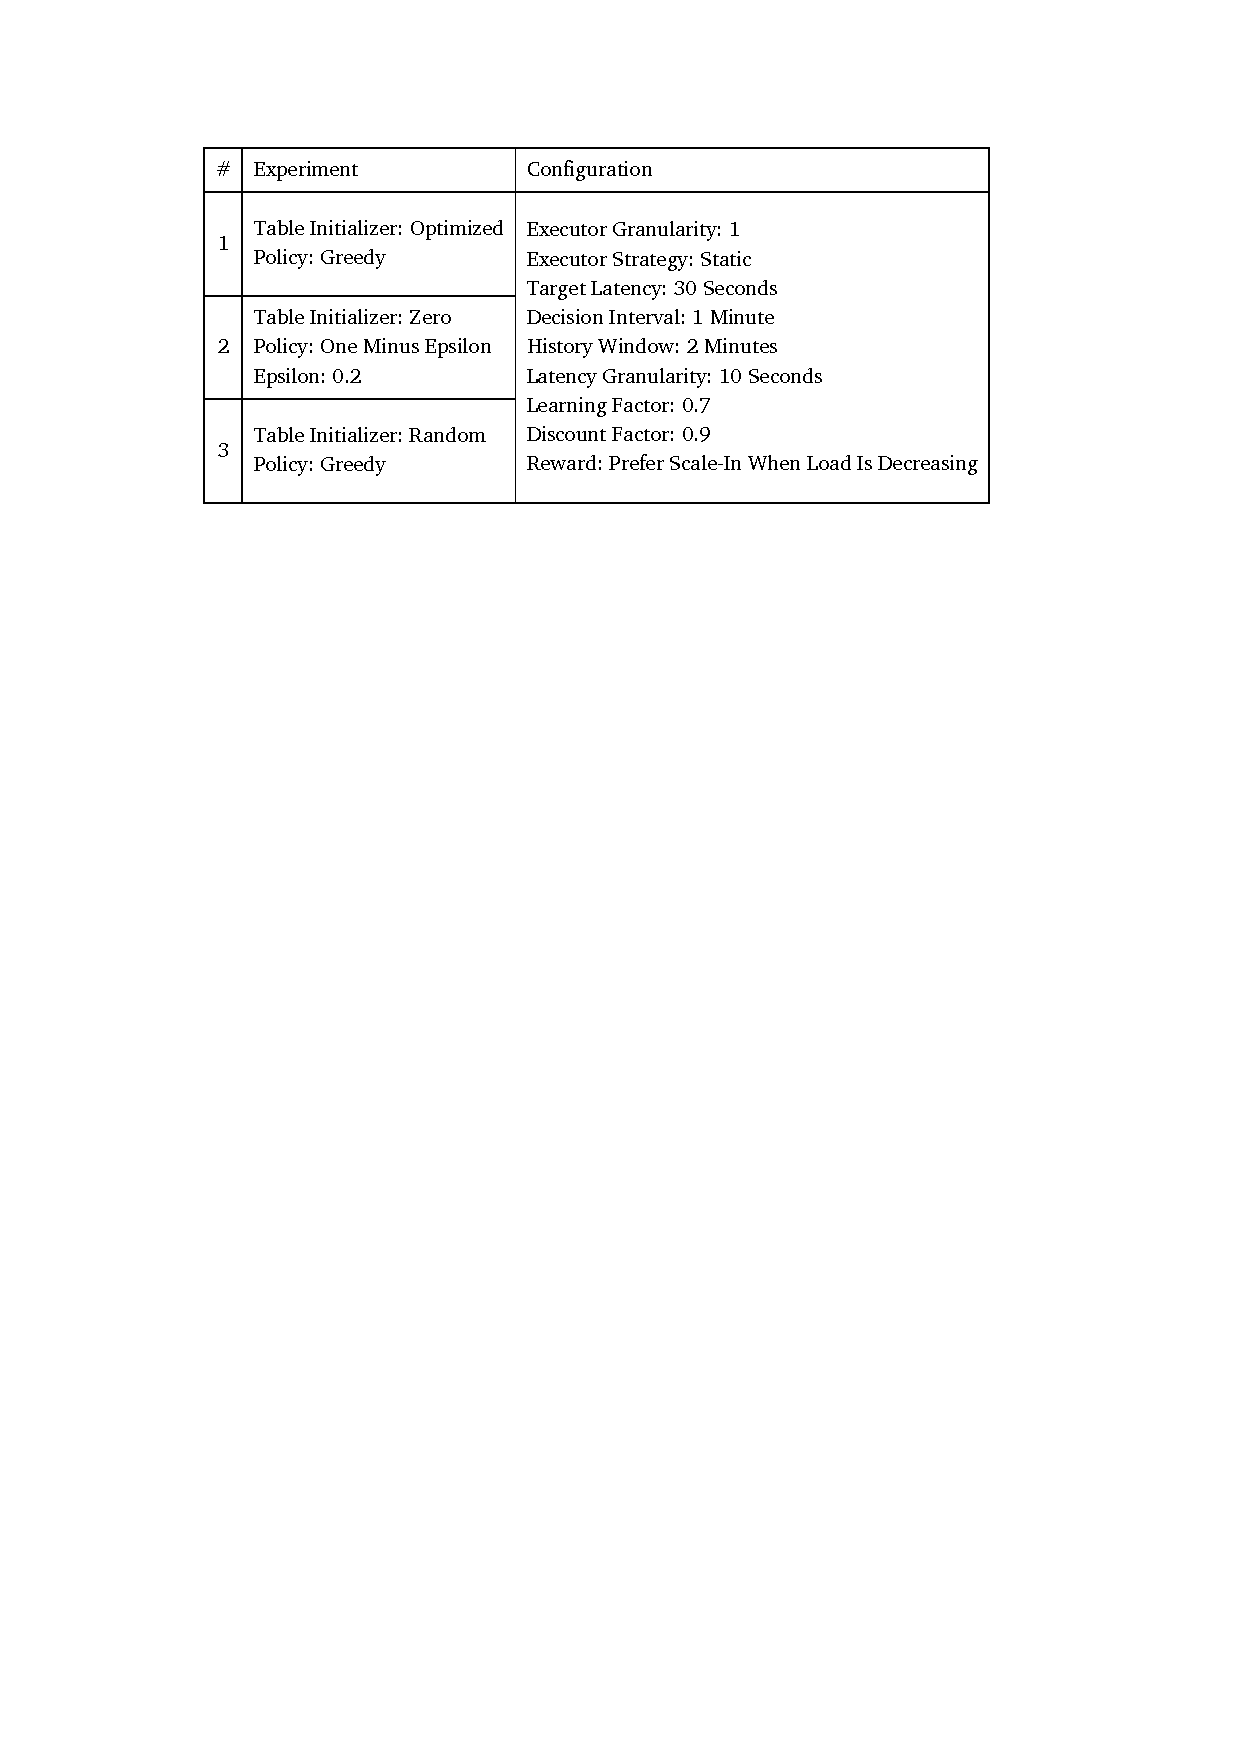
\includegraphics[clip,trim=3.3cm 21.18cm 4.1cm 2.5cm]{tables/ex4.pdf}
    \centering
    \caption{State Space Initializer Configuration Parameters}
    \label{eval:tab:ex4}
\end{table}

Figures~\ref{eval:f:e4:w1:lat},~\ref{eval:f:e4:w1:lat-c},~\ref{eval:f:e4:w1:exec} and ~\ref{eval:f:e4:w1:exec-c} illustrates latency and executor charts for Workload 1. Figures~\ref{eval:f:e4:w2:lat},~\ref{eval:f:e4:w2:lat-c},~\ref{eval:f:e4:w2:exec} and~\ref{eval:f:e4:w2:exec-c} illustrates latency and executor charts for Workload 2.

\begin{figure}[!htbp]
    \centering
    \begin{gnuplot}[terminal=epslatex, terminaloptions=color colortext]
        set terminal epslatex size 16cm,7.5cm
        set key outside center top horizontal
        set datafile separator ';'
        set xdata time
        set timefmt '%H:%M:%S'
        set xr ['0:00:00':'1:00:00']
        set yr [0:250]
        set xtics '00:00:00',600 nomirror
        set ytics 0,30 nomirror
        set y2r [0:250]
        set y2tics 0,30
        set samples 50000 
        unset mxtics
        unset mytics
        set grid ytics lc rgb "#bbbbbb" lw 1 lt 0
        set grid xtics lc rgb "#bbbbbb" lw 1 lt 0
        unset xl
        set yl 'Latency (Seconds)'
        plot 'ex/e4/w1/latency.csv' using 1:2 w l lc 'red' lw 4 smooth csplines t 'Optimized',\
        '' using 1:3 w l lc 'blue' lw 4 smooth csplines t 'Zero',\
        '' using 1:4 w l lc 'black' lw 4 smooth csplines t 'Random'
    \end{gnuplot}
    \caption{State Space Initializer -- Workload 1 -- Latency}
    \label{eval:f:e4:w1:lat}
\end{figure}
\begin{figure}[!htbp]
    \centering
    \begin{minipage}[h]{\linewidth}
        \centering
        \begin{gnuplot}[terminal=epslatex, terminaloptions=color colortext]
            set terminal epslatex size 16cm,7.5cm
            set key outside center top horizontal
            set datafile separator ';'
            set key width -12
            set xr [0.5:3.5]
            set yr [0:250]
            set ytics 0,30 nomirror
            set y2r [0:250]
            set y2tics 0,30
            set boxwidth 0.3 absolute
            set style fill empty
            set grid ytics lc rgb "#bbbbbb" lw 1 lt 0
            set grid xtics lc rgb "#bbbbbb" lw 1 lt 0
            unset xl
            set yl 'Latency (Seconds)'
            plot 'ex/e4/w1/latency-c.csv' using 1:2:3:4:5:xticlabels(7) with candlesticks lc 'black' lw 4 t 'Min/Max/Percentiles',\
            '' using 1:6:6:6:6 with linespoints pt 5 lc 'black' lw 4 t 'Average',\
            30 dashtype 2 lc 'black' lw 4 t 'Target'
        \end{gnuplot}
        \caption{State Space Initializer -- Workload 1 -- Latency}
        \label{eval:f:e4:w1:lat-c}
    \end{minipage}\hfil
    \begin{minipage}[h]{\linewidth}
        \centering
        \begin{gnuplot}[terminal=epslatex, terminaloptions=color colortext]
            set terminal epslatex size 16cm,7.5cm
            set key outside center top horizontal
            set datafile separator ';'
            set xdata time
            set timefmt '%H:%M:%S'
            set xr ['0:00:00':'1:00:00']
            set yr [2:26]
            set y2r [2:26]
            set ytics 0,4 nomirror
            set xtics '00:00:00',600 nomirror
            set y2tics 0,4
            unset mxtics
            unset mytics
            set grid ytics lc rgb "#bbbbbb" lw 1 lt 0
            set grid xtics lc rgb "#bbbbbb" lw 1 lt 0
            unset xl
            set yl 'Number of Executors'
            plot 'ex/e4/w1/exec.csv' using 1:2 w l lc 'red' lw 4 t 'Optimized',\
            '' using 1:3 w l lc 'blue' lw 4 t 'Zero',\
            '' using 1:4 w l lc 'black' lw 4 t 'Random'
        \end{gnuplot}
        \caption{State Space Initializer -- Workload 1 -- Number of Executors}
        \label{eval:f:e4:w1:exec}
    \end{minipage}\hfil
    \begin{minipage}[h]{\linewidth}
        \centering
        \begin{gnuplot}[terminal=epslatex, terminaloptions=color colortext]
            set terminal epslatex size 16cm,7.5cm
            set key outside center top horizontal
            set datafile separator ';'
            set xr [0.5:3.5]
            set yr [2:26]
            set y2r [2:26]
            set ytics 0,4 nomirror
            set y2tics 0,4 nomirror
            set boxwidth 0.3 absolute
            set style fill empty
            unset xl
            set grid ytics lc rgb "#bbbbbb" lw 1 lt 0
            set grid xtics lc rgb "#bbbbbb" lw 1 lt 0
            set yl 'Number of Executors'
            plot 'ex/e4/w1/exec-c.csv' using 1:2:3:4:5:xticlabels(7) with candlesticks lc 'black' lw 4 t 'Min/Max/Percentiles',\
            '' using 1:6:6:6:6 with linespoints pt 5 lc 'black' lw 4 t 'Average' 
        \end{gnuplot}
        \caption{State Space Initializer -- Workload 1 -- Number of Executors}
        \label{eval:f:e4:w1:exec-c}
    \end{minipage}
\end{figure}
\begin{figure}[!htbp]
    \centering
    \begin{minipage}[h]{\linewidth}
        \centering
        \begin{gnuplot}[terminal=epslatex, terminaloptions=color colortext]
            set terminal epslatex size 16cm,7.5cm
            set key outside center top horizontal
            set datafile separator ';'
            set xdata time
            set timefmt '%H:%M:%S'
            set xr ['0:00:00':'1:00:00']
            set yr [0:170]
            set y2r [0:170]
            set xtics '00:00:00',600 nomirror
            set ytics 0,20 nomirror
            set y2tics 0,20
            unset mxtics
            unset mytics
            set samples 50000 
            unset xl
            set grid ytics lc rgb "#bbbbbb" lw 1 lt 0
            set grid xtics lc rgb "#bbbbbb" lw 1 lt 0
            set yl 'Latency (Seconds)'
            plot 'ex/e4/w2/latency.csv' using 1:2 w l lc 'red' lw 4 smooth csplines t 'Optimized',\
            '' using 1:3 w l lc 'blue' lw 4 smooth csplines t 'Zero',\
            '' using 1:4 w l lc 'black' lw 4 smooth csplines t 'Random'
        \end{gnuplot}
        \caption{State Space Initializer -- Workload 2 -- Latency}
        \label{eval:f:e4:w2:lat}
    \end{minipage}\hfil
    \begin{minipage}[h]{\linewidth}
        \centering
        \begin{gnuplot}[terminal=epslatex, terminaloptions=color colortext]
            set terminal epslatex size 16cm,7.5cm
            set key outside center top horizontal
            set datafile separator ';'
            set key width -12
            set xr [0.5:3.5]
            set yr [0:410]
            set y2r [0:410]
            set ytics nomirror
            set y2tics 0,50
            set ytics 0,50
            set boxwidth 0.3 absolute
            set style fill empty
            unset xl
            set grid ytics lc rgb "#bbbbbb" lw 1 lt 0
            set grid xtics lc rgb "#bbbbbb" lw 1 lt 0            
            set yl 'Latency (Seconds)'
            plot 'ex/e4/w2/latency-c.csv' using 1:2:3:4:5:xticlabels(7) with candlesticks lc 'black' lw 4 t 'Min/Max/Percentiles',\
            '' using 1:6:6:6:6 with linespoints pt 5 lc 'black' lw 4 t 'Average',\
            30 dashtype 2 lc 'black' lw 4 t 'Target'
        \end{gnuplot}
        \caption{State Space Initializer -- Workload 2 -- Latency}
        \label{eval:f:e4:w2:lat-c}
    \end{minipage}\hfil
    \begin{minipage}[h]{\linewidth}
        \centering
        \begin{gnuplot}[terminal=epslatex, terminaloptions=color colortext]
            set terminal epslatex size 16cm,7.5cm
            set key outside center top horizontal
            set datafile separator ';'
            set xdata time
            set timefmt '%H:%M:%S'
            set xr ['0:00:00':'1:00:00']
            set yr [2:26]
            set y2r [2:26]
            set xtics '00:00:00',600 nomirror
            set ytics 0,4 nomirror
            set y2tics 0,4
            unset mxtics
            unset mytics
            unset xl
            set grid ytics lc rgb "#bbbbbb" lw 1 lt 0
            set grid xtics lc rgb "#bbbbbb" lw 1 lt 0     
            set yl 'Number of Executors'
            plot 'ex/e4/w2/exec.csv' using 1:2 w l lc 'red' lw 4 t 'Optimized',\
            '' using 1:3 w l lc 'blue' lw 4 t 'Zero',\
            '' using 1:4 w l lc 'black' lw 4 t 'Random'
        \end{gnuplot}
        \caption{State Space Initializer -- Workload 2 -- Number of Executors}
        \label{eval:f:e4:w2:exec}
    \end{minipage}
\end{figure}
\begin{figure}[!htbp]
    \centering
    \begin{gnuplot}[terminal=epslatex, terminaloptions=color colortext]
        set terminal epslatex size 16cm,7.5cm
        set key outside center top horizontal
        set datafile separator ';'
        set xr [0.5:3.5]
        set yr [2:26]
        set ytics 0,4 nomirror
        set y2r [2:26]
        set y2tics 0,4
        set boxwidth 0.3 absolute
        set style fill empty
        unset xl
        set grid ytics lc rgb "#bbbbbb" lw 1 lt 0
        set grid xtics lc rgb "#bbbbbb" lw 1 lt 0  
        set yl 'Number of Executors'
        plot 'ex/e4/w2/exec-c.csv' using 1:2:3:4:5:xticlabels(7) with candlesticks lc 'black' lw 4 t 'Min/Max/Percentiles','' using 1:6:6:6:6 with linespoints pt 5 lc 'black' lw 4 t 'Average' 
    \end{gnuplot}
    \caption{State Space Initializer -- Workload 2 -- Number of Executors}
    \label{eval:f:e4:w2:exec-c}
\end{figure}
\FloatBarrier
\subsection{Conclusion}

For Workload 1 as depicted, optimized initializer beats zero and random initializers and to a large degree it is able to respect target latency. For Workload 2, random initializer performs similar to optimized initializer. But this is only achieved by chance. Looking at Figure~\ref{eval:f:e4:w2:exec} reveals two pieces of information.
\begin{itemize}
    \item Since the first part of Workload 2 is not intensive and Auto-Scaler is running with minimum executors, random initializer performs early Scale-Out -- there is no other option with minimum executors. Since this action helps to improve the latency, Auto-Scaler learns this bit of information and performs another Scale-Out which in turn improves latency further. Up until the workload reaches critical point -- in terms of latency -- Auto-Scaler has already performed consecutive Scale-Out actions which helps to diverge faster. Note that if the workload begins with a peak -- just like Workload 1, there is little chance that random initializer could win the game.
    \item Considering final stage of workload, where Auto-Scaler has removed so many executors that the latency started to increase fast -- Figure~\ref{eval:f:e4:w2:lat} -- which indicates state space still contains wrong information. Note that optimized initializer removes executors at a slower rate.
\end{itemize}

Looking at behavior of zero initializer reveals an interesting point. Since Auto-Scaler has started with minimum executors, it wasn't able to process the workload. On the other hand all states are initialized to zero. Thus, Auto-Scaler will stick to No-Action -- with a probability of $\epsilon$ will perform random action. Staying with No-Action leads to even higher latency which is a new state initialized with zero. Again, Auto-Scaler will stick to No-Action which in turn increases latency and causes Auto-Scaler to land in another new state. This process keeps going -- latency increases leading Auto-Scaler to land in a new state. This means, Auto-Scaler never sees the previous states to utilize learned information. This is the point where Queue-Aware executor strategy could potentially help to complement Auto-Scaler's actions. In case Auto-Scaler is behind schedule and by any chance takes a random Scale-Out action, Queue-Aware strategy adds a batch of executors at once which would considerably improve latency.

In general, if an Auto-Scaler starts with zero or random initializer, it is better to start with maximum -- or at least reasonable -- number of executors such that initial random actions don't cause serious SLO violations.

\clearpage
\section{Experiment 5: Learning Factor}